\subsection*{Explicación}
Para este ejercicio hice uso del if statement de verilog para comprobar cada caso aunque tambíen pude hacer uso del case statement (pero preferí el if).
\subsection*{Código}
\faGithub \space
\href{https://github.com/warleon/Arch-lab1/tree/master/pregunta3}{https://github.com/warleon/Arch-lab1/tree/master/pregunta3}\\
make comparador

%\subsection*{Tabla de verdad}

%\subsection*{Mapa de Karnaugh}

%\subsection*{Ecuaciones booleanas}

\subsection*{Resultados}
\begin{figure}[h]
    \centering
    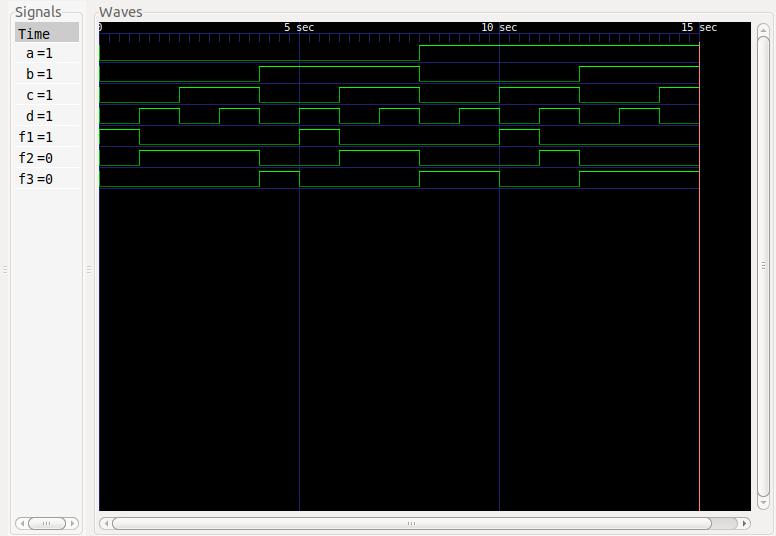
\includegraphics[scale=0.6]{fotos/resultados/arki-COMPARADOR.png}
    \caption{waves comparador}
\end{figure}